\documentclass[aspectratio=169, table]{beamer}
\usepackage[utf8]{inputenc}
\usepackage[T1]{fontenc}
\usepackage{graphicx}
\usepackage{fontspec} 
\usepackage{xcolor}
\usepackage{tcolorbox}
\usepackage{listings} % Add the listings package

\setsansfont[
ItalicFont=fonts/TitilliumWeb-Italic.ttf,
BoldFont=fonts/TitilliumWeb-Bold.ttf,
BoldItalicFont=fonts/TitilliumWeb-BoldItalic.ttf,
]{TitilliumWeb-Regular.ttf}

\subtitle{IF140303: Web-based Application Development}
\title{\Huge {\textbf{01: \\HTML}}}
\date[Serial]{\scriptsize {PRU/SPMI/FR-BM-18/0222}}
\author[Pradita]{\small {\textbf{PRADITA UNIVERSITY}}}

\usetheme{Pradita} %To change Styles of the ppt

\begin{document}
\begin{frame}
		\titlepage
	\end{frame}
	
	\begin{frame}{Goals}
		\vskip-1cm
		\begin{itemize}
			\item To learn about computers and programming
			\item To understand the basics of HTML and web development
			\item To create and style web pages using HTML and CSS
			\item To learn how to structure content on a web page with HTML elements
		\end{itemize}
	\end{frame}

	\begin{frame}{Introduction to HTML}
		\vskip-0.5cm
		\begin{itemize}
			\item HTML (HyperText Markup Language) is the standard markup language for creating web pages and web applications.
			\item It defines the structure and layout of a web page using a system of markup tags and attributes.
			\item HTML documents consist of a series of elements, each represented by a pair of tags, such as `<p>` for paragraphs or `<h1>` for headings.
			\item Elements can contain text, images, multimedia, and other types of content.
		\end{itemize}
	\end{frame}

	\begin{frame}[fragile] % Add the 'fragile' option here
		\frametitle{Basic HTML Structure}
		\vskip0.5cm
		\begin{lstlisting}[language=HTML]
<!DOCTYPE html>
<html>
<head>
    <title>My First HTML Page</title>
</head>
<body>
    <h1>Hello, World!</h1>
    <p>This is my first HTML page.</p>
</body>
</html>
		\end{lstlisting}
	\end{frame}

	\begin{frame}{HTML Elements}
		\begin{tcolorbox}[standard jigsaw, opacityback=0, opacityframe=0, sharp corners, boxrule=0pt]
					\textbf{\textcolor{white}{HTML elements are the building blocks of web pages. Here are some common HTML elements:}}
					\begin{itemize}
						\item `<h1>`, `<h2>`, `<h3>`... - Headings
						\item `<p>` - Paragraphs
						\item `<a>` - Links
						\item `<img>` - Images
					\end{itemize}
		\end{tcolorbox}
	\end{frame}

	\begin{frame}[fragile]{HTML Code - Part 1}
		\begin{verbatim}
		<!DOCTYPE html>
		<html lang="en">
		<head>
		    <meta charset="UTF-8" />
		    <meta name="viewport" content="width=device-width, initial-scale=1.0" />
		    <title>Document</title>
		    <link rel="stylesheet" href="assets/css/reset.css" />
		    <link rel="stylesheet" href="assets/css/converter.css" />
		</head>
		<body>
		\end{verbatim}
	\end{frame}
	
	\begin{frame}[fragile]{HTML Code - Part 2 (First)}
\begin{verbatim}
<div class="container">
  <div class="left-section">
    <h1>Currency Converter</h1>
    <div class="amount-wrapper">
      <label for="amount">Amount</label>
      <input type="number" id="amount" />
    </div>
    <div class="converter-wrapper">
      <div class="from-converter-wrapper">
        <label for="from">From</label>
\end{verbatim}
\end{frame}

\begin{frame}[fragile]{HTML Code - Part 2 (Second)}
\begin{verbatim}
<select name="from" id="from">
          <option value="gbp">IDR - Indonesia Rupiah</option>
          <option value="usd">USD - United States Dollar</option>
          <option value="eur">EUR - Euro Member Countries</option>
          <option value="gbp">GBP - United Kingdom Pound</option>
        </select>
      </div>
      <div class="buttons">
        <button id="reverse">Reverse</button>
      </div>
\end{verbatim}
\end{frame}

\begin{frame}[fragile]{HTML Code - Part 2 (Third)}
\begin{verbatim}
      <div class="to-converter-wrapper">
        <label for="to">To</label>
        <select name="to" id="to">
          <option value="gbp">IDR - Indonesia Rupiah</option>
          <option value="usd">USD - United States Dollar</option>
          <option value="eur">EUR - Euro Member Countries</option>
          <option value="gbp">GBP - United Kingdom Pound</option>
        </select>
      </div>
    </div>
    <div class="buttons">
      <button id="convert">Convert</button>
    </div>
  </div>
\end{verbatim}
\end{frame}

\begin{frame}[fragile]{HTML Code - Part 3}
\begin{verbatim}
  <div class="right-section">
    <!-- Label for result -->
    <div class="result-wrapper">
      <label class="result">$ 100</label>
      <label class="currency">USD</label>
    </div>
    <div class="result-wrapper">
      <label class="result">Rp 1.500.000</label>
      <label class="currency">IDR</label>
    </div>
    <label class="exchange-rate">1 USD = 15.000 IDR</label>
  </div>
</div>
</body>
</html>
\end{verbatim}
\end{frame}

% \begin{frame2}
%     \frametitle{References}
%     \begin{tcolorbox}[standard jigsaw, opacityback=0, opacityframe=0, sharp corners, boxrule=0pt]
%         \begin{columns}[T] %T for Top, C for Center, B for Bottom
%             \begin{column}{0.7\textwidth}
%                 Jain, H. (2017). Problem Solving in Data Structures \& Algorithms Using C++: Programming Interview Guide.
%             \end{column}
%             \begin{column}{0.3\textwidth}
%                 
%             \end{column}
%         \end{columns}
%     \end{tcolorbox}
% \end{frame2}


\begin{frame3}
		\vskip1cm
		\begin{tcolorbox}[standard jigsaw, opacityback=0, opacityframe=0, sharp corners, boxrule=0pt]
			\begin{columns}[T] %T for Top, C for Center, B for Bottom
				\begin{column}{0.5\textwidth}
					\textbf{\textcolor{white}{HTML elements are used to describe the structure and content of a web page. Each element has a specific purpose and can contain other elements or text. By combining different elements, you can create complex and interactive web pages.}}
				\end{column}
				\begin{column}{0.5\textwidth}
					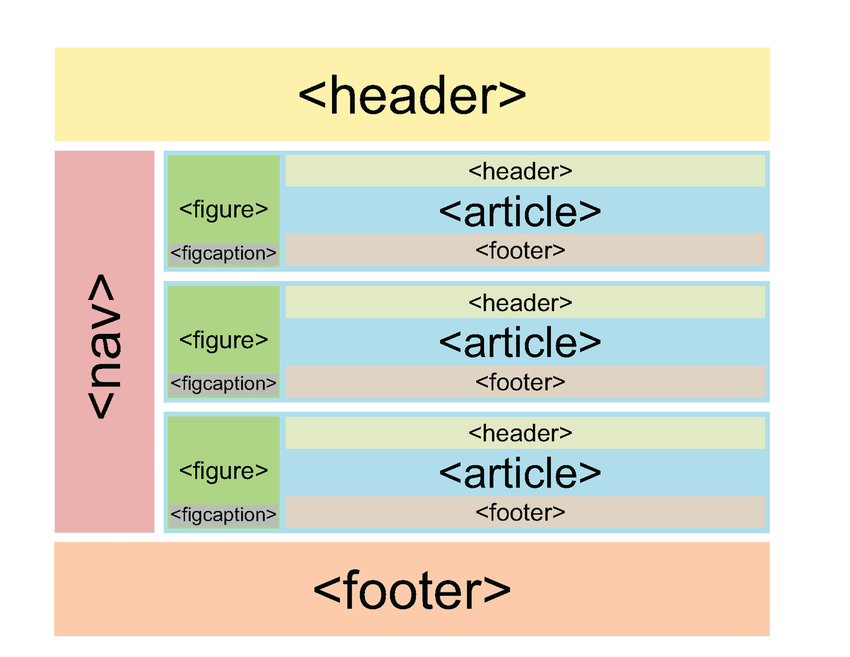
\includegraphics[width=1\textwidth]{classFiles/html_structure.png}
				\end{column}
			\end{columns}
		\end{tcolorbox}
	\end{frame3}

\begin{frame4}
	\frametitle{Thank You}
\end{frame4}

\end{document}
